\documentclass[11pt, a4paper]{article}

%\usepackage[T1]{fontenc}
%\usepackage{fullpage}

\usepackage[utf8]{inputenc} % comment when using lualatex
\usepackage[italian]{babel} % lingua e a-capo-sillabato
\usepackage{graphicx}
\usepackage[hidelinks]{hyperref} % link di pagina
\usepackage[bottom]{footmisc} % note appiccicate al fondo della pagina
\usepackage{float} % per posizionamento immagini
\usepackage{amsthm} % per ambienti stile teorema
\usepackage{tabularx} %tabelle
\usepackage[table]{xcolor} %colore caselle
\usepackage{enumitem} %additional commands for lists
\usepackage{fancyhdr}
\usepackage[font=footnotesize,labelfont=bf]{caption} % small caption font-size



\pagestyle{fancy}
\fancyhf{}% Clear header/footer
\fancyhead[C]{\footnotesize\textit{Documento:} D3 \hfill SleepCode \hfill \textit{Versione:} 1.0}
\renewcommand{\headrule}{{\color{red!70}\rule{\textwidth}{2pt}}}
\setlength{\headheight}{22pt}

\renewcommand\UrlFont{\color{blue}\rmfamily} % colore link

\theoremstyle{definition} % stile dei newtheorem (non italizzati)
\newtheorem{funcreq}{RF} %% numerazione dei requisiti funzionali
\newtheorem{nonfuncreq}{RNF} %% requisiti non funzionali
\newtheorem{backend}{BE}
\newtheorem{frontend}{FE}




\title{Documento di Architettura}

\author{Raffaele \textsc{Castagna}\\
Alberto \textsc{Rovesti}\\
Zeno \textsc{Saletti}}

\newcommand{\groupNumber}{G17}

% Web address for the project (if any)
% \newcommand{\homepage}{\url{https://www.}}

% data
\date{\today}

\makeatletter{}

% IL PREAMBOLO FINISCE QUI %%%%%%%%%%%%%%%%%%%%%%%%%%%%%%%%%%%%%%%%%%%%%%%%%%%%



\begin{document}

% La pagina di copertina si trova in un file .tex a parte
% NON MODIFICARE QUESTO COMANDO!!!
\begin{titlepage}
\newcommand{\HRule}{\rule{\linewidth}{0.3mm}} % Defines a new command for horizontal lines, change thickness here
\center % Centre everything on the page

%------------------------------------------------
%	Logo
%------------------------------------------------

\includegraphics[width=0.3\textwidth]{materiale/UniTrento_logo_ITA_colore.png}\\[0.5cm]
%------------------------------------------------
%	Headings
%------------------------------------------------
\textsc{\Large Dipartimento di Ingegneria\\e Scienza dell'Informazione}\\[1.5cm]

{\Huge\textbf{Sleep Code}}\\[0.5cm]
\textsc{\large Progetto per il Corso di Ingegneria del Software}\\
\textsc{\large Anno Accademico 2023-2024}\\[0.5cm]

%------------------------------------------------
%	Title
%------------------------------------------------

\HRule\\[0.4cm]
{\huge\bfseries \@title}\\[0.1cm]
\HRule\\[1cm]

\begin{minipage}{\textwidth}
\begin{flushleft}
\textit{Descrizione:} documento di analisi dei requisiti funzionali, non funzionali, front-end e back-end.
\end{flushleft}
\end{minipage}\\[1.5cm]


\begin{minipage}{0.4\textwidth}
\begin{flushleft}
\large
\textit{Numero documento:} D1
\end{flushleft}
\end{minipage}
\begin{minipage}{0.4\textwidth}
\begin{flushright}
\large
\textit{Versione documento:} 2.4
\end{flushright}
\end{minipage}\\[1.5cm]

%------------------------------------------------
%	Author(s)
%------------------------------------------------
\begin{minipage}{0.4\textwidth}
\begin{flushleft}
\large
\textit{Membri del gruppo:}\\
\@author % Your name
\end{flushleft}
\end{minipage}
~
\begin{minipage}{0.4\textwidth}
\begin{flushright}
\large
\textit{Numero gruppo: }
\groupNumber
\end{flushright}
\end{minipage}

% 	If you don't want a supervisor, uncomment the two lines below and comment the code above
% 	{\large\textit{Author(s)}}\\
% 	\@author % Your name

%------------------------------------------------
%	Date
%------------------------------------------------

\vfill\vfill
\textit{Ultima revisione:}
{\@date}

\end{titlepage}

\tableofcontents

\newpage

\section*{Scopo del documento}
In questo documento viene riportata la definizione dell'architettura del
progetto \textit{SleepCode} impiegando diagrammi delle classi, realizzati
secondo gli standard di Unified Modeling Language (UML), e codice Object
Constraint Language (OCL). Nel documento precedente (D2, \textit{Specifica
dei Requisiti}) sono stati presentati il diagramma degli use case, quello
di contesto e infine il diagramma dei componenti. Considerando tale
progettazione, viene ora definita l'architettura del sistema specificando
in modo più dettagliato le classi che dovranno essere implementate sotto forma di
codice, insieme alla logica che regola il comportamento del software che
si intende realizzare.

Il linguaggio UML, utilizzato per descrivere le classi, è supportato da
codice OCL, impiegato invece per specificare gli aspetti logici citati sopra
che non sarebbero esprimibili formalmente mediante i soli diagrammi delle
classi.


\newpage
\section{Diagramma delle classi}
Nella presente sezione vengono illustrate in linguaggio UML le classi
previste dal progetto \textit{SleepCode}. Ogni componente del diagramma
dei componenti, presente nel documento D2, viene qui rappresentato
in forma di una o più classi. Le classi individuate sono costituite
da un nome, un insieme di attributi che identificano i dati gestiti dalla
classe stessa e una lista di metodi che definiscono le operazioni
eseguibili da quella classe. Eventuali relazioni tra classi sono evidenziate
da alcune associazioni.

\subsection{Utenti}
L'attore che nel diagramma di contesto usufruisce delle funzionalità offerte
dal servizio è l'utente. Come descritto nei documenti di Analisi dei Requisiti (D1)
e Specifica dei Requisiti (D2), esistono tre categorie di utenti: anonimo, autenticato
e amministratore.

Dal momento che tutte queste categorie condividono alcune funzionalità, è stata
creata una classe \texttt{Utente}, che logicamente corrisponde alla categoria
degli utenti anonimi, ovvero utenti che non hanno effettuato il login. Di fatto,
non è prevista la memorizzazione di alcuna informazione riguardo a questa categoria
di utenti (non sono previsti attributi), e le uniche operazioni disponibili sono:
\begin{itemize}
    \item \texttt{login()}: richiesta di accesso.
    \item \texttt{signUp()}: richiesta di registrazione.
    \item \texttt{recuperaAccount()}: richiesta di avvio della procedura di recupero account.
\end{itemize}
Da questa prima classe viene definita, mediante generalizzazione, la classe
\texttt{UtenteAutenticato}, che aggiunge metodi e attributi accessibili previo
login:
\begin{itemize}
    \item \texttt{user\_id}: dal momento che email e password dell'account di sistema
    possono essere modificate dall'utente autenticato, la classe contiene questo
    attributo con ruolo di identificatore univoco.

    \item \texttt{username, email, password}: i dati richiesti per creare un
    account. In caso di autenticazione con Google, è richiesto che la classe
    memorizzi solo l'indirizzo email impiegato.

    \item \texttt{isGoogle}: parametro che distingue gli account collegati con
    Google da account registrati con il meccanismo di credenziali interne.

    \item \texttt{risolti[*]}: insieme che raccoglie gli identificatori dei problemi
    risolti dall'utente.

    \item \texttt{preferiti[*]}: insieme degli identificatori dei problemi
    contrassegnati come preferiti, da parte dell'utente.

    \item \texttt{logout()}: richiesta di logout.
    
    \item \texttt{setEmail, setPassword}: procedure utili a modificare le credenziali
    dell'account. Oltre alle nuove credenziali, viene richiesta, per questioni di sicurezza,
    la password attualmente in uso. Entrambi i metodi restituiscono una risposta
    di tipo booleana per segnalare il successo o l'insuccesso delle rispettive operazioni.

    \item \texttt{setPreferito}: questo metodo provvede ad aggiungere o
    eliminare dalla lista dei preferiti dell'utente il problema fornito: se
    presente, il suo identificatore viene rimosso dalla lista, altrimenti
    viene aggiunto.

    \item \texttt{getPreferiti}: affinché l'utente possa vedere i preferiti
    della sua lista, questo metodo permette di restituire questo dato.

    \item \texttt{getNumeroRisolti, getRisoltiPerDifficolta}: questi metodi
    permettono di fornire informazioni riguardo ai progressi dell'utente.
\end{itemize}
Infine, un'ulteriore generalizzazione specifica le funzionalità aggiuntive
dell'utente amministratore, ovvero metodi utili alla gestione dei problemi
disponibili nel catalogo:
\begin{itemize}
    \item \texttt{aggiungiProblema}
    \item \texttt{modificaProblema}
    \item \texttt{eliminaProblema}
\end{itemize}
Nella Figura \ref{utenti} sono mostrate in linguaggio UML le classi
sopra descritte.

\begin{figure}[H]
\centering
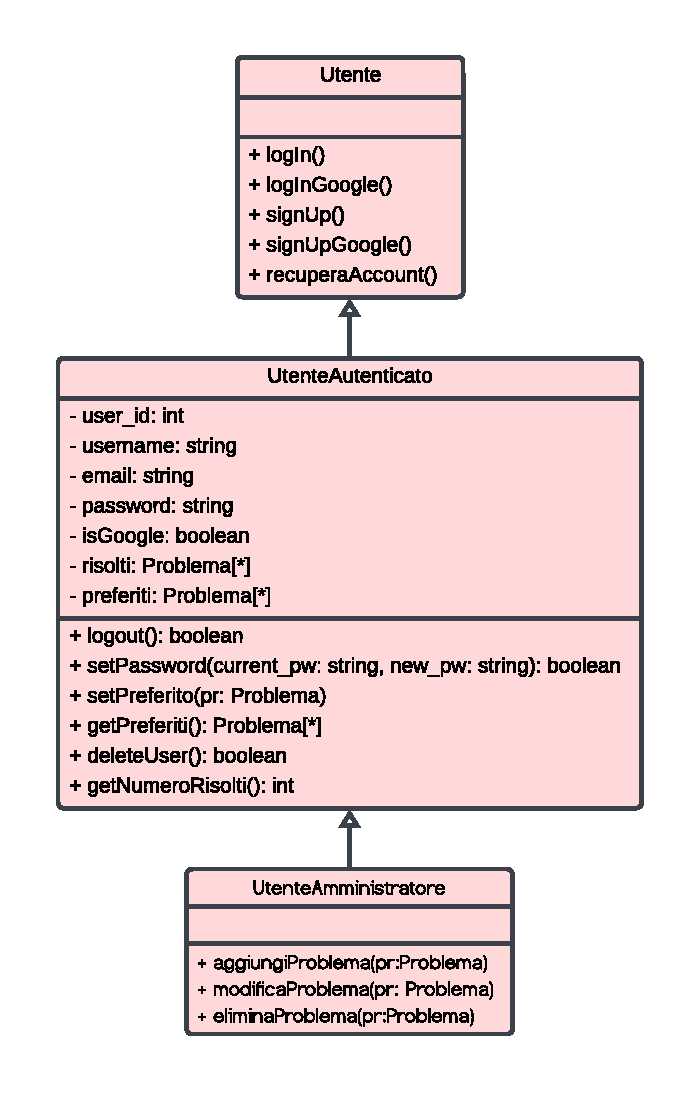
\includegraphics[scale = 0.7]{materiale/class-utenti.pdf}
\caption{Definizione della classe \texttt{Utente}}
\label{utenti}
\end{figure}







\newpage
\subsection{Gestione autenticazione}
Nel diagramma di contesto, l'autenticazione si avvale di due sistemi
subordinati: \textit{Firebase DB}, che si occupa di memorizzare gli account
registrati con sistema di autenticazione interno, e \textit{Google SignIn},
con il quale è possibile, per un utente, effettuare la registrazione o
l'autenticazione mediante un account Google.

Il componente \textit{Gestione Autenticazione} del rispettivo diagramma si
occupa di interagire con tali sistemi esterni in modo da convalidare le
operazioni di registrazione e autenticazione. Per questo motivo, nel diagramma
delle classi viene individuata la classe \texttt{Autenticazione}:
\begin{itemize}
    \item \texttt{autorizzato}: questo attributo mantiene lo stato dell'autorizzazione
    dell'utente
    \item \texttt{isGoogle}:
    \item \texttt{registraAccount}: questo metodo esegue la registrazione
    comunicando con il servizio di database.
    \item \texttt{autentica}: l'autenticazione mediante credenziali interne
    avviene grazie a questo metodo.
    \item \texttt{registraGoogle}
    \item \texttt{autenticaGoogle}
\end{itemize}
Tutti i metodi comunicano all'esterno l'esito delle loro operazioni mediante
un valore booleano di ritorno.


\newpage
\section{Codice in Object Constraint Language}
Nella sezione che segue viene descritta formalmente la logica prevista
nel comportamento di alcune classi, in relazione alle loro operazioni
possibili. Il codice OCL impiegato consente di esprimere tale logica,
non descrivibile con i soli diagrammi delle classi in UML.


\section{Diagramma delle classi con codice OCL}
In Figura \ref{umlocl} è riportato un diagramma che mostra nell'insieme
sia le classi individuate che il relativo codice OCL.

\begin{figure}[H]
\centering
%\includegraphics[options]{name}
\caption{Diagramma delle classi arricchito dal codice OCL}
\label{umlocl}
\end{figure}

\end{document}